%&&&&&&&&&&&&&&&&&&&&&&&&&&&&&&&&&&&&&&&&&%
%% Übungsblattvorlage					  %
%%% written by Andreas Rain				  %
%&&&&&&&&&&&&&&&&&&&&&&&&&&&&&&&&&&&&&&&&&%

\documentclass[fleqn, oneside, 10pt, titlepage]{report}
%
%Zeichensatz UTF-8 und T1-Zeichensatz
\usepackage[utf8x]{inputenc} 
\usepackage[T1]{fontenc}
%\newcommand{\changefont}[3]{\fontfamily{#1}\fontseries{#2}\fontshape{#3}\selectfont}
% 

%Silbentrennung nach neuer deutscher Rechtschreibung
%\usepackage[ngerman]{babel} % Neue Rechtschreibung
%
%Einige Mathe-Symbole aus AMS-LaTeX
\usepackage{amsmath,amssymb,euscript}
%
% schönere Aufzählungen
\usepackage{enumerate}
%
% Für Bilder 
\usepackage{graphicx}
\usepackage{float} % lädt das Paket zur Verwendung von zusätzlichen Positionsbefehlen

%Graue box
\usepackage{framed}
\usepackage{xcolor}

\definecolor{MyBoxColor}{rgb}{0.9,0.9,0.9}
\newenvironment{shadedSmaller}{
  \def\FrameCommand{\fboxsep=\FrameSep \colorbox{MyBoxColor}}
  \MakeFramed {\advance\hsize-2\width\FrameRestore}}
{\endMakeFramed}

\newenvironment{shadedSmallerPadding}{
  \def\FrameCommand{\fboxsep=0.3cm \colorbox{MyBoxColor}}
  \MakeFramed {\advance\hsize-1.1\width\FrameRestore}}
{\endMakeFramed}
%%%%%%%%%%%%%%%%%%%%%%%%%%

% Standard Font auf Überschriften übernehmen.
%\usepackage{sectsty}
%\sectionfont{\fontfamily{pag}\fontseries{b}\fontsize{13pt}{20pt}\selectfont}
%\subsectionfont{\fontfamily{pag}\fontseries{b}\fontsize{11pt}{20pt}\selectfont}
%\subsubsectionfont{\fontfamily{pag}\fontseries{b}\fontsize{10pt}{20pt}\selectfont}
%\paragraphfont{\fontfamily{pag}\fontseries{b}\fontsize{11pt}{20pt}\selectfont}
%\subparagraphfont{\fontfamily{pag}\fontseries{b}\fontsize{10pt}{20pt}\selectfont}

%
% Farben und die Code-Umgebung einbinden
%
\usepackage{listings, color}
%
% Ein paar Standardfarben
\definecolor{darkblue}{rgb}{0,0,.6}
\definecolor{darkred}{rgb}{.6,0,0}
\definecolor{darkgreen}{rgb}{0,.6,0}
\definecolor{red}{rgb}{.98,0,0}
%
%Standardmäßig Java vorher laden
\lstloadlanguages{Java}
\lstloadlanguages{SQL}
% Standard-Layout für die Code-Umgebung (alle Sprachen)
\lstset{%
	language=SQL,
 	basicstyle=\footnotesize\ttfamily,
	showspaces=false,
	showtabs=false,
	columns=fixed,
	frame=none,
	numberstyle=\tiny,
	breaklines=true,
	showstringspaces=false,
	xleftmargin=0cm,
	tabsize=4,
	keywordstyle=\color{darkblue},
	commentstyle=\color{darkred},
	stringstyle=\color{darkgreen},
	emph={i, t, a, f},
	emphstyle=\color{red}
}%

%
% Seitenranddefinitionen
%   Links etwas mehr Rand als rechts, damit sich die Zettel später besser abheften lassen.
\usepackage[a4paper]{geometry} 
\geometry{a4paper,tmargin=2.5cm, bmargin=3cm, lmargin=3cm, rmargin=3cm, headheight=3em, headsep=1em, footskip=1cm} 

%
% Kopf- und Fußzeilendefinition
%
\usepackage{fancyhdr}
\pagestyle{fancy}
\fancyhf{}
%


% Oben rechts die Namen der Teilnehmer der Gruppe
%
%Oben Links das Fach und darunter die Nummer des Übungsblattes
\fancyhead[L]{\textcolor{gray}{HPSN Summary}}
%
% Die Übungsgruppe oben in der Mitte (momentan auskommentiert)
%\fancyhead[C]{Gruppe 2}
%
%Fußzeile mittig die Seitenzahl
\fancyfoot[C]{\textcolor{gray}{Seite \thepage}}
%
% Fußzeile links das aktuelle Datum (alternativ kann hier der Abgabetag eingetragen werden)
\fancyfoot[L]{\textcolor{gray}{\today}}

%Fancy Table
\usepackage{tabularx}
\usepackage{booktabs}
\usepackage{colortbl}
\usepackage{tikz}
\usetikzlibrary{calc}
\pgfdeclarelayer{background}
\pgfdeclarelayer{foreground}
\pgfsetlayers{background,main,foreground}
%

%
% Deutsche Absatzformatierung: Zwischen zwei Absätzen eine Zeile (1em) frei und 
% kein Einrücken der ersten Zeile
%
\setlength{\parskip}{1em}
\setlength{\parindent}{0pt}

%Titelseite
\title{\Large HPSN Summary}


%
% Beginn des Dokumentes
%
\begin{document}
\maketitle %Ausgabe der Titelseite 
\newpage
\tableofcontents
\newpage

\chapter{Introduction} \label{CHAP:Introduction}

\section{Motivation for High Performance Systems and Networks}

Some laws to remember:

\begin{description}
	\item[Moore's Law] For transistors: The amount of transistors doubles every two years. \\
	Similar observations can be found for Network Capacity, Storage, HDD Rates and more.
	
	\item[Wirth's law] Software becomes slower more rapidly than hardware becomes faster.
	
	\item[Gate's law] Speed of software halfs every 18 months.
	
	\item[May's law] Software efficiency halves every 18 months, compensating Moore's Law.
\end{description}

High performance and efficient network technologies are especially important for Embedded devices, HPCs, High Performance Routers and Real-time applications.\\

Therefore the lecture covers following subjects:

\begin{itemize}
	\item Micro-optimization in Chapter \ref{CHAP:MOPT}
	\item Performance Evaluation in Chapter \ref{CHAP:PERFEVAL}
	\item Algorithms and Datastructures and degree of freedom utilization in Chapters \ref{CHAP:PRINCIPLES} and following chapters.
\end{itemize}

\textbf{Examples of problems} this lecture tries to solve/highlight:\\

Different types of systems may have different bottlenecks, i.e., for

\textit{Network endnodes}:

\begin{itemize}
	\item Specialized for computations, General-purpose, i.e. endnode bottlenecks usually result from \textit{structure} and \textit{scale}
	\item \textbf{Structure}: \textit{Layered structure} of Operating systems, \textit{protection mechanisms} to protect the OS from other applications, core OS routines are written using \textit{general mechanisms} (Schedulers, Allocators). The combination of the different mechanisms may slow down networking software.
	
	\item \textbf{Scale}: Scaling factors of thousands of clients are possible, where many OSs simply don't use efficient enough data structures and algorithms, since they were designed for small amounts of connections.
\end{itemize}

In the book the following table shows a mapping between bottlenecks and solutions:

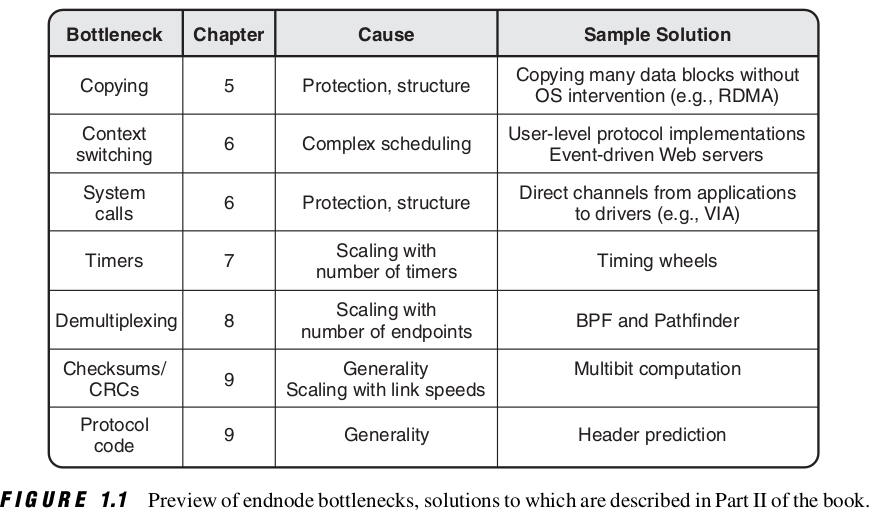
\includegraphics[width=.8\textwidth]{images/chap1/endnode_bottlenecks}

\textit{Router Bottlenecks}:

\begin{itemize}
	\item Special-purpose device, problems caused by \textit{scale} and \textit{services} and not structure
	
	\item {\textbf{Scale}: i.e., \textit{bandwidth scaling (from 1Gbps to 40Gbps)} and \textit{population scaling (growing number of endpoints)}}
	
	\item {\textbf{Services}: Many QOS (for instance \textit{network guarantees)} are/have been added over time, s.a., congestion control, protection during attacks, availability..}
\end{itemize}

Again, a mapping of bottlenecks to solutions provided by the book:

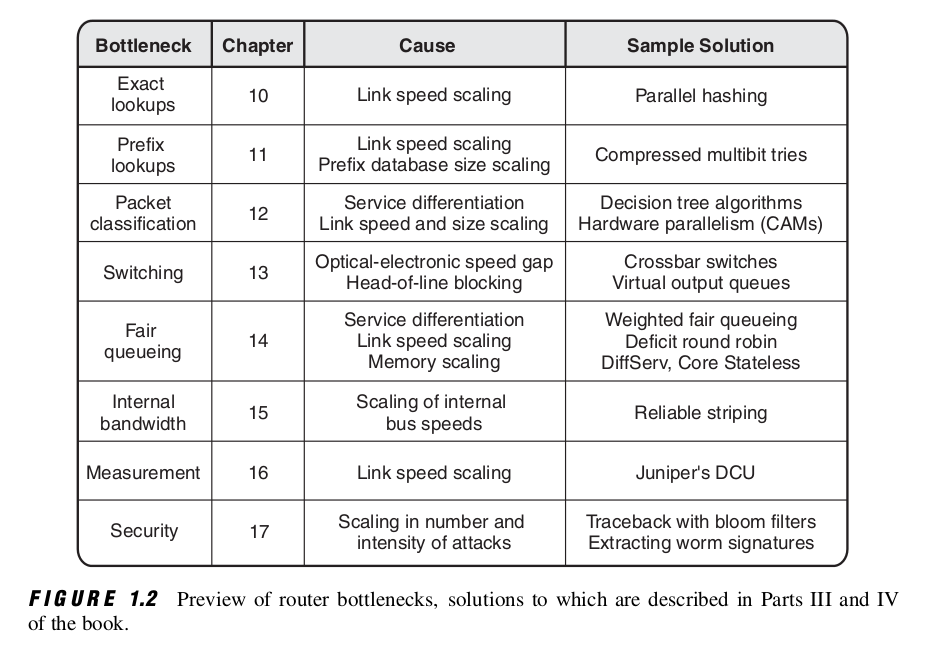
\includegraphics[width=.8\textwidth]{images/chap1/router_bottlenecks}

Nowadays, routers provide \textit{service differentation}, i.e., handling different packets differently, depending on the offered services, which requires \textit{packet classification}.

\section{Warmup-Example: Scenting an evil packet}

\textbf{Problem:} An attacker tries to include malicious data in a packet, that is later executed on the target system. How? If the target system does not allocate enough buffer space and does not check
for overflow, malicious code can be performed on the target system.

\textbf{Solution:} Implemenation of a pre-filter by estimating what a packet "usually" \ looks like, i.e., estimating the frequencies of bytes in a packet.

Issues regarding the implementation:

\begin{itemize}
	\item Fast counting of characters/bytes in a packet
	\item Estimation of non-malicious packet
	\item Estimating such that false negatives don't appear. False positives are ok, since they have to go through the IDS.
\end{itemize}

\textbf{Stage 1 - Strawman Soltuion:} naive approach, consists of an array $C$ with 256 elements, one for each byte. For incoming packets $\rightarrow$ iteration through data, increment $C$ at position of byte.
A threshold array $T$ is used to estimate whether $C$ is out of the ordinary. In formulas:

$$C[j] \geq L \cdot T[j] , L = packet \ length, j \in \mathbb{N}, 0 \leq j \leq 255$$

The example in the book only applies for HTTP headers, i.e., the check is only done on the URL and is only initiated if a HTTP Header is recognized.

Usually packets are incoming at high speed and ideally they are processed before the next one arrives. This is called \textbf{wire speed processing}!

Since intialization of arrays is static we have 1 write + 1 read per $C$ and 1 read per $T$ we have at least 768 operations per packet. However, a packets minimum size is 40 bytes and in this case we have a great overhead.

\textbf{Stage 2 - Thinking Algorithmically:} Only keep track of the largest ratio of character count to threshold. I.e., $C[k]/T[k] = MAX$ is being memorized. New characters still increment $C[i]$ and if $C[i]/T[i] > MAX$, max is replaced. The process can stop if $MAX > L$.

\textbf{Stage 3 - Exploit Hardware:} The last loop is eliminated, but we still have division. Idea: approximate threshold by a power of 2, as they are estimates anyway. Then shifting can be used instead of division.
For instance 1/29 becomes 1/32. Shift values are now stored instead of thresholds themselves. Now $C[i]$ is incremented an the check is $C[i] << T[i] > MAX$.

Still one read + write for $C$ and one read for $T$ is required, which is now the new bottleneck instead of computation itself. By combining the counter and threshold into one word only one read is required (for instance using a union).


\textbf{Stage 4 - Cleaning Up:} Intialization is still done for 256 values. Hence, lazy init. is preferable, since for packets of 40 bytes, less operations are needed. Idea:

Keep a register $G$ (3-bit as we already have 29 bit for $C$ and $T$ and therefore 3 left). When a new packet is incoming increment a global register $g mod 8$. When $C[i]$ is incremented, check if $G[i] == g$, if that is not the case, we know that $i$ was not used in this turn and can be initialized to $1$, otherwise it's incremented.



























\chapter{Micro-Optimization} \label{CHAP:MOPT}

\section{Counting bits}

\textbf{Question 1:} How many bits are set to one?

\textbf{Solution 1.1:} Simple approach 

Walk through every bit, if bit is one increase counter.

\begin{lstlisting}[language=C]
#define MAXBITS 32

int countBits(unsigned int x) { 
  int bits = 0; 
  for (int i = 0; i < MAXBITS; i++) { 
    if (((1<<i) & x) != 0) bits++; 
  } 
  return bits; 
}
\end{lstlisting}

\textit{Improvements:}

\begin{itemize}
\item Loop reversal
\begin{lstlisting}[language=C]
for (int i = MAXBITS-1; i>=0; i--)
\end{lstlisting}

\item Condition to computation
\begin{lstlisting}[language=C]
bits += (x >> i) & 1; 
\end{lstlisting}

\item Index removal
\begin{lstlisting}[language=C]
bits += (x & 1); 
x >>= 1; 
\end{lstlisting}

\item Loop inversion

\item Delay slot

\item Loop unrolling
\end{itemize}





\textbf{Solution 1.2:} Kerninghan bit clearing

\begin{lstlisting}[language=C]
int countBits(unsigned int x) { 
  int bits = 0; 
  while (x != 0) { 
    x = x & (x-1); 
    bits++; 
  } 
  return bits; 
}
\end{lstlisting}

\textbf{Solution 1.3:} Magic

\begin{lstlisting}[language=C]
int countBits(unsigned int x) { 
  return ((x * 0x000200040008001ULL) & 0x111111111111111ULL) % 0xf; 
}
\end{lstlisting}



\textbf{Question 2:} Is the number of bits set odd?

\textbf{Solution 2.1:} Halve \& Remove pairs
\begin{lstlisting}[language=C]
int bitCountIsOdd(unsigned int x) { 
  x ^= x >> 16; 
  x ^= x >> 8; 
  x ^= x >> 4; 
  x ^= x >> 2; 
  x ^= x >> 1; 
  return x & 1; 
}
\end{lstlisting}

\textbf{Solution 2.2:} Lookup table

Tradeoff between operation minimization and table size.
\begin{lstlisting}[language=C]
int bitCountIsOdd(unsigned int x) { 
  static unsigned char parity[] = { 
    0,1,1,0, 1,0,0,1, 
    1,0,0,1, 0,1,1,0 }; 
  x ^= x >> 16; 
  x ^= x >> 8; 
  x ^= x >> 4; 
  x &= 0xf; 
  return parity[x]; 
}
\end{lstlisting}

\textit{Improvement:} Inline bitmap
\begin{lstlisting}[language=C]
return (0x6996 >> x) & 1; 
\end{lstlisting}





\section{Block Parity}

Given n blocks of size SIZE each: Calculate block $n+1$ (d) such that every bit is the XOR of the matching bits in the other blocks.

\begin{lstlisting}[language=C]
#define SIZE 512

void blockParity(char *d, char **s, int n) { 
  for (int i = 0; i < SIZE; i++)
    d[i] = 0; 
  
  for (int j = 0; j < n; j++) { 
    for (int i = 0; i < SIZE; i++) {
      //Calculate block by block
      d[i] ^= s[j][i]; 
    }
  } 
}
\end{lstlisting}

\textit{Improvements:}
\begin{itemize}
\item Words\footnote{''A word is basically a fixed-sized group of digits that are handled as a unit by the instruction set or the hardware of the processor.'' (wikipedia)}
\item loop reversal
\item loop interchange
\item register (skip initialization)
\end{itemize}

\begin{lstlisting}[language=C]
#define WORDS 128

void blockParity(int *d, int **s, int n) { 
  for (int i = WORDS-1; i >= 0; i--) { 
    int t = s[0][i] ^ s[1][i];
    
    for (int j = 2; j < n; j++) {
      // Calculate bit by bit
      t ^= s[j][i]; 
    }
    
    d[i] = t; 
  } 
}
\end{lstlisting}

\textit{Further improvements:}

\begin{itemize}
\item Loop unrolling
\item Loop specialization
\end{itemize}

\begin{lstlisting}[language=C]
#define WORDS 128 

void blockParity(int *d, int **s, int n) { 
  switch (n) { 
    case 2: for (int i = WORDS-2; i>=0; i -= 2) 
              d[i] = s[0][i] ^ s[1][i];
              d[i+1] = s[0][i+1] ^ s[1][i+1]; 
            break; 
    case 3: for (int i = WORDS-2; i>=0; i -= 2) 
              d[i] = s[0][i] ^ s[1][i] ^ s[2][i];
              d[i+1] = s[0][i+1] ^ s[1][i+1] ^ s[2][i+1]; 
            break; 
    case ...
  } 
}
\end{lstlisting}

\begin{shadedSmaller}
\textbf{Summary:} Loop optimizations

\begin{description}
\item[loop reversal] \lstinline|i++ --> i--|
\item[index removal] \lstinline|p[i] --> p++|
\item[loop inversion] \lstinline|while --> do-while|
\item[loop unrolling] \lstinline|for(;;) x --> x;x;x;...|
\item[loop interchange] \lstinline|for(i;;) for(j;;) --> for(j;;) for(i;;)|
\item[loop unswitching] \lstinline|for(;;) if --> if for(;;) else for(;;)|
\end{description}
\end{shadedSmaller}

\begin{shadedSmaller}
\textbf{Summary:} Generic optimizations

\begin{description}
\item[condition to computation] \lstinline|if() x=... -> x=x+y| 
\item[lookup table] \lstinline|t[x]|
\item[inline bitmap] \lstinline|(t >> x) & mask|
\item[software pipelining] Group independent tasks, so that a processor with multiple instruction units can execute them in parallel. Do not confuse with hardware/processor pipelining. \lstinline|A(1)B(1)A(2)B(2) --> A(1)A(2)B(1)B(2)|
\item[instruction sharing] reuse instructions (e.g. by jump label)
\item[function call inlining] Replace function call with function body
\item[register usage] 
\end{description}
\end{shadedSmaller}

\textbf{int64x4 vs. int64x8} ???

\textbf{int64x4 vs. sse2x4} The int64 algorithms are cache-polluting\footnote{''Cache pollution describes situations where an executing computer program loads data into CPU cache unnecessarily.'' (wikipedia)}. This makes them slightly faster, but slowing the rest of the machine down. 




\section{One's complement checksum}

Used in IPv4 to calculate the header checksum.

\textit{Algorithm:} 
\begin{enumerate}
\item Add the first two 16-bit values
\item\label{carry} Add carry bit to result
\item Add the next 16-bit value
\item Go to \ref{carry}, until all values are added
\item Take one's complement (invert all bits)
\end{enumerate}

\section{Coffee shop}

Error-handling strategies for loosely coupled systems:

\begin{description}
\item[Write-off] Do nothing, or discard what you've done.

\item[Retry] Retry the one that failed.

\item[Compensating action] Undo the one that failed

\item[Transaction coordinator] Coordinator prepares action and commit only if both systems are ready.
\end{description}

\chapter{Performance Evaluation} \label{CHAP:PERFEVAL}

Scientifically sound work often requires an evaluation of data and results as well as generating reproducible results.

This chapter covers things that need to be considered in order to create a scientifically sound evaluation.

\section{Methods of Evaluation}

\begin{itemize}
    \item Measurement of a real system (hard without disturbing the system)
    \item Simulation (Discrete Events, Simulated Time, Side effects are hard to simulate)
    \item Analytical (Models and Numerical)
\end{itemize}

Some terms: \textbf{Load} - Different systems may have different workloads, which has significant impact on the results (also the patterns in which load appears).

\textbf{Metric} - The measurement that is to be captured in the experiment. No general form of performance metrics - i.e., can be aggregations and so on. Different aggregations on performance measurements may be of interest, i.e.,

\begin{itemize}
    \item average
    \item 95-percentile (order list, take element at 95\%)
    \item worst case
\end{itemize}

for metrics like datarate, response time, energy consumption and many more.

\textbf{Scientific Method for Performance Evaluation}

\begin{enumerate}
    \item Define Hypothesis
    \item Design Experiment
    \item Validate
    \item Satisfied? No $\rightarrow$ repeat
    \item Validation OK
\end{enumerate}

The process has to be \textbf{repeatable}, \textbf{independently verifiable} and \textbf{conclusions independent of point of view or bias}.

\textbf{Goals of Performance Evaluation}

\begin{itemize}
    \item Comparison - Vary design parameters and compare their influence on the performance, also consider different design alternatives
    \item System Dimensioning - Determining size of components
\end{itemize}

For comparison a well-defined work load model is needed, but the exact value of intensity is not needed. For system dimensioning on the other hand, an estimate of the intensity of work load is needed, which is why the results highly depend on that estimate.

\subsection{Factors}

Different factors have influence on the outcome of the result. As state load is one of them. There may be other factors (also known as parameters or predicator variables) to the experiment that may vary results and need to be considered.

Some possible factors: Background Activity, Multiple Users, Network Activity (Operating System comparison).

\textbf{Different System Designs for Factors}

\begin{itemize}
    \item Simple - Start typical configuration, vary parameters at a time and pick best, may give false conclusions
    \item Full Factorial - Every possible combination of factors, can find every effect and interaction between factors, repetitions needed for validity and repeatability, cost of application is too high very quickly.
    \item Fractional factorial - A fraction of all factor combinations, Calculate contributions of factors to total variance and choose, Disadvantage: Indicates interactions among some but not all factors;\\ For example $2^k$-design (only 2 possibilities for every factor) 
\end{itemize}

Additional notes (book):

\begin{description}
    \item[Hidden Factor Paradox] Hidden factors may invalidate results, for instance analyzing throughput / speed in network data and ignoring buffer sizes in use. Proper randomization may rid of some of the hidden factors.
    \item[Simpson's Paradox] Performance metric is success probability. Example: Interested in whether a mobile will reach more than 1.5Mbit/s, hence success if this is the case. Ignoring buffer size, the example in the book shows that fast mobiles have a higher success rate. However, when considering the different buffer sizes (small, large) slow mobiles actually have a higher success probability (Book Page 7 to 8).
\end{description}

\subsection{Example SuperDHT}

Data structure to find documents in a fast manner. Supposedly fast.. Documents are mapped to $[0,1]$ square node closest cartesian distance.

Geographical basis: Nodes map longitude and latitude to $[0,1]$ square links.

\textbf{Measurement:} Simple - Take one measurement, plot, look at conclusion. Problems?: Not reproducible and has no meaning.

Advanced - Take $x_1, \dots, x_n$ independent measurements and obtain average $\mu$, plot, look at conclusion. Problem? (Mean is) Still not reproducible or significant, consider \textit{"Then there is the man who drowned crossing a stream with an average depth of six inches"}.

Solution - Take the confidence interval as well. Reason: Simulations with random components require confidence intervals.

Advanced 2 - $x_1, \dots , x_n$ measurements, test if it fits normal distribution (simple gaussian ..), if so apply t-test, else increase sample size $n$.

\textbf{Central limit theorem} - \textit{Sum of a large number of independent observations from any distribution converges towards a normal distribution}.

\subsection{Performance Patterns}

Some traits are common among performance measurements and therefore should be known (\textit{performance patterns}). (not included in the lecture but in the book).

\textbf{Bottlenecks} - many systems performances are dictated by their weakest components

\textbf{Congestion Collapse} - Congestion appears when intensity of load exceed system capacity. Congestion is unavoidable, but congestion collapse should be avoided, which is reduction of system utility on increasing loads.

\textbf{Competition Side Effect} - Performance of a user may have effects on that of other users on a system, a paradox when providing more resources makes performance for users worse. Cause for this is, increasing resources for some users will take away resources for competing users, worsening their performance.

\textbf{Latent Congestion Collapse} - Large complex systems may have several bottlenecks. Removing a bottleneck (by adding more resources) may have a contradictory effect and lead to congestion collapse.

\subsection{Check-list}

The book states a check-list of its own for performance evaluation which may be worth remembering:

\begin{enumerate}
    \item Define goal
    \item Identify factors
    \item Define metrics
    \item Define offered load
    \item Know your bottlenecks
    \item Know your system well
\end{enumerate}

\textbf{Scientific method check list:}

\begin{enumerate}
    \item Hypothesis, Design Experiments, Validate until validation is fine
    \item Quantify accuracy of your results (95-percentile etc.)
    \item Make findings reproducible, define assumptions..
    \item Remove what can be removed
\end{enumerate}

\section{Analysis and Comparison}

\subsection{Students-t test}

Check whether a small set of samples is likely to originate from a normal distribution. Need to specify confidence intervals (for one sided tests 5\% means 95\% of the data is within the distribution, for two sided 5\% has the same meaning, but 2.5\% on the left and 2.5\% on the right).

\subsection{Q-Q Plot}

In some cases data that may seem to have a correlation may not actually have one. The Q-Q-plot calculates a scatter plot over the percentiles of data for multiple dimensions. It does not try to show correlation between data, but rather correlations between their distributions, i.e. a linear line along the diagonal shows high correlation between the distributions of the data.

\subsection{Distributions}

\textbf{Uniform} - given a set of attributes and samples, a sample has the same probability to have a certain attribute for all attributes.

\textbf{Gaussian} - Also called bell curve, based on the standard deviation and mean of data. Usually the "95\%" include two times the standard deviation, the rest is outside and unlikely to appear within samples.

\subsection{Models}

Models are used to provide simplified explanations of observations of real data. For instance, regressions are models into which data is fitted. For this least squares is widely used for error minimization. In this case, we implicitly assume that error terms are gaussian with equal variance, which may be false. An alternative is to use Laplacian distribution.

\textbf{iid} - Independence assumption, i.e., "Independent and identically distributed" - assumption is a property of a model and not of the data itself. When working with models, we often assume independence and identical distribution, although this may not be the case.

\textbf{Regression} - a model of a curve that is estimated over a set of samples.
Statistical tests are used to verify whether the calculated model is actually good.

Gneral formular for linear regression $y = a + bx$, then the regression can be calculated using $$b = \dfrac{\sum_{n=1}^{N} (x_n - \overline{x})(y_n - \overline{y})}{\sum_{n=1}^{N} (x_n - \overline{x})^2}$$ and $a = \overline{y} - b \overline{x}$.

In general you can have more predictor variables, extending the formular by those variables..

\subsection{Correlation and Causation}

Data that seems to have a correlation may not always have a causation. A simple example is the comparison of deaths over 10 years by any means correlated to beared growth of individuals. That data may have a correlation, but it is highly unlikely that there is a causation as well.

\subsection{Interpolation and Sampling}

When sampling data at a certain frequency/rate, the sampling has to be performed at twice the frequency/rate of the highest frequency/rate. Although, there are cases where this is not the case, in general aliasing is introduced into the sampled data set.

\section{Conclusions}

Awareness of what constitutes you scientific experiments, whether simulation, measurement or analytical conclusions have to be structured, reproducible and so on...

Good foundation in statistics and performance evaluation is a requirement for good quality analysis in networks and high performance systems.
























\chapter{The Principles} \label{CHAP:PRINCIPLES}

\section{The fifteen principles}

The 15 principles are demonstrated on the ternary CAM \textbf{(content-addressable memory)} problem:

Overview:

\begin{tabular}{|c|c|c|}
\hline 
\textbf{Number} & \textbf{Principle} & \textbf{Used in} \\ 
\hline 
P1 & Avoid obvious waste & Zero-copy interfaces \\ 
\hline 
P2 & Shift computation in time &  \\ 
P2a & Precompute & Application device channels \\ 
P2b & Evaluate lazily & Copy-on-write \\ 
P2c & Share expenses, batch & Integrated layer processing \\ 
\hline 
P3 & Relax requirements &  \\ 
P3a & Trade certainty for time & Stochastic fair queuing \\ 
P3b & Trade accuracy for time & Switch load balancing \\ 
P3c & Shift computation in space & IPv6 fragmentation \\ 
\hline 
P4 & Leverage off system components &  \\ 
P4a & Exploit locality & Locality-driven receiver \\
P4b & Trade memory for speed & Processing; Lulea IP lookups \\
P4c & Exploit existing hardware & Fast TCP checksum \\
\hline 
P5 & Add hardware &  \\ 
P5a & Use memory interleaving and pipelining & Pipelined IP lookups \\ 
P5b & Use wide word parallelism & Shared memory switches \\ 
P5c & Combine DRAM and SRAM effectively & Maintaining counters \\ 
\hline 
 &  & \textbf{Networking examples} \\ 
\hline 
P6 & Create efficient specialized routines & UDP Checksums \\ 
\hline 
P7 & Avoid unnecessary generality & Fbufs \\ 
\hline 
P8 & Don't be tied to reference implementation & Upcalls \\ 
\hline 
P9 & Pass hints in layer interfaces & Packet filters \\ 
\hline 
P10 & Pass hints in protocol headers & Tag switching \\ 
\hline 
P11 & Optimize the expected case & Header prediction \\ 
P11a & Use caches & Fbufs \\ 
\hline 
P12 & Add state for speed & Active VC list \\ 
P12a & Compute incrementally & Recomputing CRCs \\ 
\hline 
P13 & Opt. degrees of freedom & IP trie lookups \\ 
\hline 
P14 & Use bucket sorting, bitmaps & Timing wheels \\ 
\hline 
P15 & Create efficient data structures & Level-4 switching \\ 
\hline 
\end{tabular} 

Categorization: The principles can be divided into different subcategories,

Principles 1 to 5 are called \textbf{system principles}, 6 to 10 \textbf{Improving efficiency while retaining modularity} and 11 to 15 \textbf{speeding it up}.  

Examples for each principle:

\textbf{P1}: Look for obvious waste in the computation of similar expressions and only calculate them once. For instance $i = 5.1 * n + 2$ is calculated and later $j = (5.1 * n+ 2) *4$, which can obviously use the first result.

\textbf{P2}: Systems have aspect in space time, \textbf{space} refers to geographic distribution of subsystems, \textbf{time} refers to the fact that a system is instantiated at different time scales (fabrication time, compile time, parameter setting time, run time), shifting computation in time can lead to more efficiency.

\textbf{a)} Precompute: For instance, you have a DSP which needs to generate a sinusoidal signal. The samples of the sinusoidal can be precomputed and stored in a table.

\textbf{b)} Evalute lazily: Example is \textbf{copy on write}, only copy data when you want to perform a write operation, not before.

\textbf{c)} Share expenses: For instance \textbf{batching}, multiple expensive operations are computed together, which may be more efficient than doing them one after another.

\textbf{P3}: Relax System Requirements: Typical layered systems designed in a top-down approach divide functionalities on subsystems on different layers. This is good for abstraction but may have negative effects on efficiency.

\textbf{a)} Trade Certainty for Time: Make use of probabilities. An example is Cisco's netflow, when there is no capacity to count packets, it will count random samples and statistically extrapolate those and the count will be correct to a certain precision.

\textbf{b)} Trade Accuracy for Time: To gain efficiency you can reduce accuracy of operations in some cases. Multimedia processing often relies on lossy compressions which accuracy may be reduced to gain performance. (For instance replace divide by shift and lose a little accuracy)

\textbf{c)} Shift Computation in Space: Some subsystems may have to adapt to loose requirements introduced in other subsystems, which is called \textbf{shifting computation in space}. Example, routers need to fragment packets is avoided by having end systems calculate packet sizes that will pass all routers.

\textbf{P4}: Leverage of System components, top-down provides good modularity, partial bottom-up design may be required for performance critical applications.

\textbf{a)} Exploit locality: Memory hardware offers efficiencies if data is laid out contiguously, same sector for disks or same DRAM page for DRAM, disk-search algorithms exploit this and IP-lookup algorithms reduce lookup times by placing several keys in a wide word.

\textbf{b)} Trade memory for speed: Lulea IP-lookup uses sparse arrays that can be looked up efficiently by space-efficient bitmaps.

\textbf{c)} Exploit hardware features: \textit{Strength reduction} is used to optimize away multiplications in loops (compilers do this).

\textbf{P5}: Add hardware to improve performance, if nothing works buy new hardware, faster processor, faster and more memory and so on which may even be more cost effective than trying to solve every problem.

\textbf{a)} Use Memory Interleaving and Pipelining: From Chapter 2, Micro-opt., similar techniques are used in IP-lookups, classification and scheduling algos. 

\textbf{b)} Use wide word parallelism: Common technique in many networking designs, example is \textit{Lucent bit vector scheme}, use wide memory words that can be processed in parallel.

\textbf{c)} Combine DRAM and SRAM: SRAM expensive and fast, DRAM cheap and slow, combination of the two to get best benefit. SRAM as a cache, DRAM as database is classical. But SRAM can be used for efficient key lookups and so on, whereas the data itself lies on DRAM.

\textbf{P6}: Efficient specialized routines, specialized routines can be more efficient for specific purposes than general-purpose routines.

\textbf{P7}: Avoid unnecessary generality, remove features to gain performance (features that are almost never used). 

\textbf{P8}: Don't be tied to reference impl., reference implementations are often overspecified and also designed to clearly state what has to be done and not for efficiency.

\textbf{P9}: Pass hints in module interfaces, pass information that lets a service avoid unnecessary computation, cache lookups and so on.

\textbf{P10}: Pass hints in protocol headers, circumvent inefficiencies in message-passing parallel systems by passing hints in message headers (carry address of interrupt handler for fast dispatch of an operation).

\textbf{P11}: Optimize the expected case, should be rather obvious, heuristically determine which case appears most often and optimize it. Handle infrequent cases that require more difficult logic.

\textbf{a)} use caches: Keep data required for the computation of expected cases in cache. When an infrequent case appears where data is not in the cache, it will have to be looked up, however it should be statistically improbable.

\textbf{P12}: Add or exploit state to gain speed, add redundant information to expensive operations to speed up the process. Classical example is the use of secondary indices in databases.

\textbf{a)} Compute incrementally: Example, incremental comp. of IP checksums when only few fields change.

\textbf{P13}: Optimize degrees of freedom, using special datastructures or algorithms some degrees of freedom may be overlooked. For example, multibit trie IP lookup algorithms overlook the DoF, that the number of bits used to index a trie node can vary.

\textbf{P14}: Special techniques for finite universes such as integers, bucket sort, array looups and bitmaps may be more efficient than general purpose algorithms (for integers).

\textbf{P15}: Algorithmic techniques to create efficient data structures, in general P1 to P14 should be applied before thinking of special algorithmic techniques. But the author states that it is still worth while.

\subsection{Eight Cautionary Questions}
Questions you should ask yourself while impl. these principles for a given problem:

\begin{enumerate}
	\item Is it worth improving performance? It may not even be necessary..
	\item Is this really a bottleneck?
	\item What is the impact of this change on the rest of the system?
	\item Does initial analysis indicate significant improvement?
	\item Is it worth adding custom hardware?
	\item Can protocol changes be avoided?
	\item Do prototypes confirm the initial promise?
	\item Will performance gains be lost if the environment changes?
\end{enumerate}

\section{Principles in Action}

Concentrating on examples used in the slides here, since there are many more in the book..

\subsection{Ternary CAM}

Ternary content-addressable memory is used to speed up specific problems. For instance, router use a longest prefix match to find IP addresses of 32 bit length an hold 300.000 entries in their table. The question is, how to efficiently store and retrieve entries based on longest prefix match?

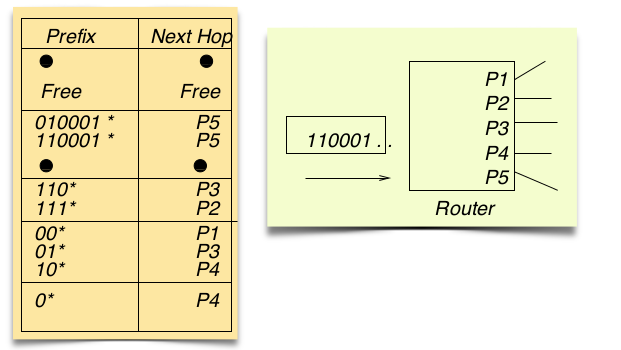
\includegraphics[width=.7\textwidth]{images/chap4/Ternary_CAM.png}

\textbf{Updating the table:} 

Ordering is done within prefixes of different length only. I.e. any \texttt{x.x.x.x/y} for constant \texttt{y} comes before \texttt{x.x.x.x/z} for $z > y$, but is not order for same addresses with prefix for \texttt{y}.

Free space is available at the beginning of the table. When an entry is inserted, holes are created by iteratively moving entries up. Starting at the top, a hole is created using the last element of prefix $i$, then proceed putting up elements for $i+k$, $i+k < 32$ and stop when a hole is available for the desired prefix length. Visually it looks as in the slides:

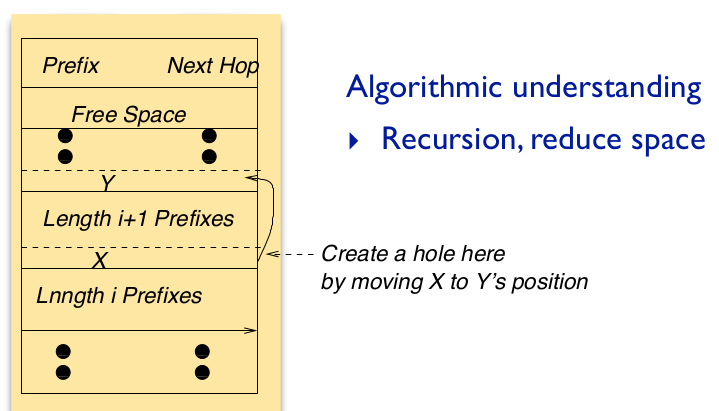
\includegraphics[width=.7\textwidth]{images/chap4/Ternary_CAM_update}

\subsection{Routing}

The Problem is, that a router wants to compute a lowest-cost path to a certain destination. In a more complex scenario, edges in the network are linked with different costs. Static routing protocols precompute paths for a router based on these link-costs and minimize path costs. Such static routing protocols are referred to as "link-state routing protocol" and routers send so called "link state packets" (LSP) that list their neighbors to all other routers.

When a router has all other LSPs, the network mapping is complete and \textbf{lowest-cost paths can be computed}, for example using \textbf{DJIKSTRA}s shortest path algorithm.

Priority queues for the link-costs are often used. However, general-purpose prio. queues such as heaps have at best a cost of $O(log N)$, leading to a complexity of $O(N log N)$ for the algorithm. Which fact can be exploited to speed up the process?

\textbf{Solution:} Since we have costs represented by small integers less than a natural number $k$ and a limited diameter (for instance, there will be no routes greater $15$ hops..), bucket sorting based priority queue can be used leading to amortized costs of $O(N + d \cdot m)$, $d = diameter, m = max \ cost$.

\subsection{LSP Fragmentation}

This was an actual problem that arose in the design of OSI and OSPF. Since routers send LSPs to all neighbors and vice versa, a lot of traffic is generated just by synchronizing routers. Packets greater the biggest MTU of 1500 bytes (at least for ethernet) have to be fragmented by routers so they are of size maximal 1500 bytes. This fragmentation is slow and expensive.

In the slide example, we have only 500 edges of 8 bytes each which is already greater than 1500 bytes. 

\textbf{Solution:} Modify Router $R1$ to be multiple routers $R1a, R1b, R1c$ with separate SQN. The set of routers connected to $R1$ is divided into multiple LSPs for pseudo-routers $R1a, \dots$ so the LSP of a pseudo-router doesn't exceed the maximal MTU. Hence, we don't have fragmentation on the network level anymore, although we fragment the packets ourselves...

Note the principal in action is \textbf{SHIFT COMPUTATION IN SPACE}!

\subsection{Quality of Service: Multicast IntServ}

Some technologies such as cable have multiple receivers listening to one connection (multicast). In the example receivers may specify which packets to receive (src/dsp address, port, protocol and so on). Therefore filters may have to be applied to huge amounts of data.

Hence the problem is

\begin{itemize}
    \item Matching against a lot of filters
    \item Multiple destinations for packets
\end{itemize}

\textbf{Solution:} Solutions include adding a field that denotes a \textbf{Flow Label}, similar to virtual circuits used in ATM.

\subsection{Resource Hogs}

Problem: Don't send packets faster than a certain rate, i.e., \texttt{B/T} bits per second.

One timer is not enough to limit the datarate, since violations of the contract are still possible. Assume, timer periods 0,T,2T,... periods having length T. Now we can have bursts ar one point in T breaking contract on a finer granularity than we measure. Hence, we need multiple timers, which on the other hand are expensive.

\textbf{Solution:} Add a random gap between the policing intervals since they need not be fixed! This way, over time, violations of contract will be encountered with a certain (by design high) probability.

\subsection{Resource Hogs Part II}

Problem: Find the user with the highest consumption, needs identification, probably some kind of sorting data structure such as priority queues.

To identify such a flow with high consumption, a statistic has to be created over many packets. It may not be sufficient to look at a time period of 5ms as some user may have micro bursts that over time don't amount to a lot of traffic.

However, creating a statistic of billions of packets with potentially thousands of different flows is expensive when performed naively.

\textbf{Solution:} \textit{Exponential (Binomial) Bucketing} of course! Relax the requirement, s.t. the accuracy can be off by a factor of 2. Aggregate users that are within a factor of 2 into the same group.

A bit in a bitmap is set if a bucket is non-empty. The resource hog is then in the bucket with the rightmost bit set. (Counting is still a problem, but another problem that is not solved here).








































\chapter{Copy Control} \label{CHAP:COPYCTL}

Since there are no slides and the copy control ex. sheet is about processes (i.e., control overhead chapter -.-, we rely on the book for this one).

\textit{Short description:} Copy control focuses on removing the obvious waste (P1) of copying when unnecessary, i.e, not imposed by hardware. Some copies such as those when an adapter receives data and forwards it to the kernel are simply necessary.

A mapping from principles to problems and solutions is given in the following table:

\begin{tabular}{|c|p{8cm}|c|}
\hline 
Number & Principle & Used in \\ 
\hline 
P13 & Memory location (on adaptor) as degree of freedom) & Afterburner \\ 
\hline 
P2b & Lazy copying using copy-on-write & Mach \\ 
\hline 
P11a and P7 & Cache VM mappings per path, Uniform fbuf space across processes & Solaris fbufs \\ 
\hline 
P10 & Pass buffer name and offset in packet & RDMA systems \\ 
\hline 
P4 & VM mapping to avoid copies in cache and apllication & Flash \\ 
\hline 
P11a & Cache VM mappings per path, Buffer sequence numbers enable checksum caching & Flash-lite \\ 
\hline 
P6 & New system call that splices I/O & Sendfile() \\ 
\hline 
P1 & Avoid repeated memory access across manipulations & ILP \\ 
\hline 
P13 & Layout code to minimize i-cache misses & x-kernel \\ 
\hline 
P13 & Layer processing order as degree of freedom & LDRP \\ 
\hline 
\end{tabular} 

\section{Why remove extra copies?}

This is kind of obvious:

\begin{itemize}
    \item It uses memory resources
    \item Takes time
\end{itemize}

Main hardware players in a server:

\begin{itemize}
    \item CPU
    \item Memory BUS
    \item I/O Bus
    \item Disk
    \item Network adaptor
\end{itemize}

Example of redundant copies in a Webserver:

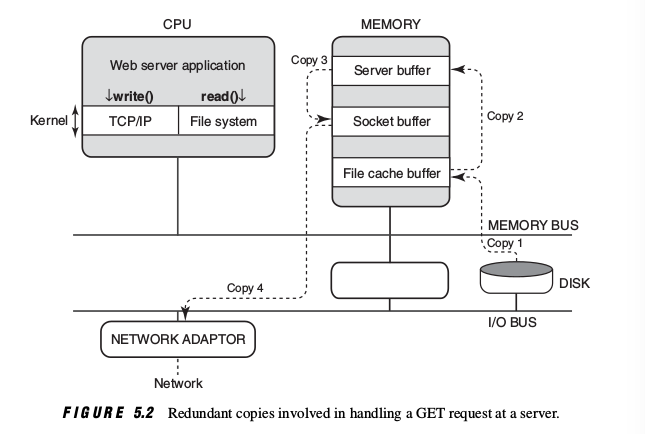
\includegraphics[width=.7\textwidth]{images/chap5/Redundant_copies}

In this example we can observe as much as 4 copies for one task.

\section{Reducing copying via local restructuring}

\subsection{Exploiting adaptor memory:} 

Memory can be located anywhere on the bus in a memory-mapped architecture. Usually, kernel memory is on memory subsystem, but there is no reason that part of it can't be on kernel (except for some security concerns -.-).

In our example, the socket buffer would now lie directly on the network adaptor and the data would be copied from the server buffer onto the socket buffer. The example in the book ignores disk-to-memory copies, which would be necessary additionally.

\textbf{Problems of this approach:}

\begin{itemize}
\item Network adaptor needs lots of memory to provide such functionality
\item Corrupted data may be written to application buffers in some cases
\item This approach may result in delayed acknowledgments (not discussed in the book but mentioned)
\end{itemize}

\subsection{Using Copy-on-Write}

We discussed this in the lecture. Copy-on-write means that an application can use memory used by another process in kernel space, as long as it doesn't write to it. When it writes data to the buffer it has to finally be copied, which may not always be the case, hence it is a good improvement.

In this case, unlike the previous solution, we want to get rid of the copy from user space to kernel space, i.e. server buffer socket buffer. (server in terms of webserver). 

\textbf{Idea:}

\begin{itemize}
    \item Replicate virtual page in memory at low cost
    \item Make the copy point to the original physical page
    \item If owner of data modifies data, OS will notice and generate two separate copies
\end{itemize}

Performance is gained under the assumption that the application does not modify it's buffer while the kernel works with it.

In our example, the buffer is represented as Server + Socket buffer in one block.

\subsection{Fbufs: Optimizing Page Remapping}

When assigning a new page in the pagemap, simply pointing to the data is not sufficient if it's owned by another page (which is mostly the case when we talk about copies).

Additional pieces of overhead that we need to take care of when copying:

\begin{itemize}
    \item Multiple-level page tables: Systems have multiple levels, thus multiple levels of pages may have to be changed.
    \item Acquiring locks and modifying page table entries: Page tables are shared resources, need protection
    \item Flushing translation look-aside buffers: Page Table Mappings are usually cache in TLB. New VP $\rightarrow$ TLB entries must be found and flushed
    \item Alloc. VM in dest. domain: Computation needed to find free page
    \item Locking the corresponding pages: Pages can be swapped to disk to make place, prevention needs locks and additional overhead.
\end{itemize}

\textbf{FBUFS Idea:} Buffer will be reused, OS can precompute page mapping information, avoids computational overhead during data transfer.

Simple way to implement is using \textit{shared memory}. Map pages $P1,\dots ,P_N$ into virtual memory tables of kernel and applications: \textbf{Bad idea!} Security violations and fault-isolation violations..

More secure: Reserve (lazy) mapped shared pages for each application-to-kernel transfer and vice versa. I.e., one set of buffer pages for FTP, one for HTTP, one for SSH and so on. OSs define multiple security domains, fbuf designers call paths sequences of security domains.

\textbf{Implementation:} Take physical pages $P1, \dots , P_k$, premap to page tables of ethernet driver, the network stack and the server (application). Reserving pages for every path can be wasteful, due to burstiness of networking, rather lazily establish mappings when paths are busy.

Network adaptor needs to quickly find which path a packet takes $\rightarrow$ \textit{early demultiplexing} (chapter 8). The adaptor has a list of free buffers, which it writes the packet to.

Additionally, designers of fbufs insisted on having it mapped onto the same VP in all applications to not have to search for it (P7, unnecessary generality).

\textit{Note:} I think more detail is unnecessary, this is enough detail. ATM the design only allows one writer and multiple readers, the book has a solution for that too.

\subsection{Transparently emulating copy semantics}

Goal: Realize (some) ideas of \textbf{fbufs}, without changing the underlying systems API. The system by Brustoloni and Steenkiste called \textbf{TCOW} (transient copy on write) should solve this problem. (Note, there has not been experimental confirmation of whether this works, as far as the book author is concerned)

\textbf{Idea:} Standard API requires possibility for applications to alloc. dealloc. buffer to kernel (fbuf makes this illegal). OS must deal with application writes and deallocations during time where kernel uses the buffer. \textit{Genie} system solves it as follows:

\textbf{Handle write threats:} \begin{itemize}
    \item When application writes, buffer is marked as read only
    \item Virtual memory fault manager is invoked
    \item If OS preserves copy-semantics, no error occurs
    \item Genie hence modifies error handler:
    \item First: For each page/buffer, keep track if outstanding sends exist (network sends)
    \item Second: Error handler makes copy of page for the application, thus preserving standard copy-semantics
    \item This technique is called \textbf{TCOW}
\end{itemize}

\textbf{Handle deallocate threats}: Normally, process exists to maintain deallocated pages in free list. Hence, daemon can also be modified to not deallocate if page is still used for sending.

In both cases, instances of \textbf{P3b}, shift comp. in space is applied, moving logic to error handler and page deallocator.

\section{Avoid copies using remote DMA}

We only talked shortly about DMA (Direct Memory Access). The idea is to let a piece of hardware directly use a buffer as if it was it's own physical memory. Workload can be taken from the CPU, which may have to chop a huge file or large packet into fragments. Instead the hardware device can write out the chunks and the application can directly use them.

\textbf{RDMA} is the idea of doing \textbf{DMA} over the network, i.e., data is transferred between two computers memories without per-packet mediation between the two CPUs. Two problems occur:

\begin{enumerate}
\item Where is received being placed?
\item Security maintenance? Just think what rogue packets with direct memory access could do ...
\end{enumerate}

\subsection{Avoid copies in a cluster}

In server clusters, for instance webservers, the need for \textbf{RDMA} may arise as data may have to be efficiently copied within the clusters servers. \textbf{VAX} Clusters, a 30 year old product from \textit{Digital Equipment Corp.} (DEC) implemented the idea of RDMA.

\textbf{Problems:} \begin{itemize}
    \item Pages need to be mapped. If Page 1,2,3 arrive in order 1,3,2 and are stored in 1,2,3 the order is broken.
    \item Remapping of large files is expensive.
\end{itemize}

\textbf{Idea for VAX:} Destination app. locks a number of physical pages. Logical view is buffer of consecutive logical pages. Sender now sends information within protocol header (buffer pos., offset..).

\subsection{Modern-Day Incarnations of RDMA}

Vax Clusters are early Storage Area Networks (SAN). Other newer technolgies include \textit{Fiber Channel}, \textit{Infiniband} and \textit{iSCSI}.

\section{Broadening to File Systems}

The last section for copy-control, as I think that we've talked about file copying and file systems as well.
The previous improvements were made to get rid of copies between applications and the network while sending data.

\subsection{Shared Memory} Unix provides system call \texttt{mmap()} that maps a file to virtual memory and other OSs provide similar functions. In theory, when mapped, it's as if a cached copy is in memory (redundant because file system also cache files). Using virtual memory, the file is only a set of mappings, and applications, file server cache and so on, can gain access to pages for the file.

\subsection{IO-Lite: Unified view of buffering}

Using \texttt{mmap()}, copies of dynamically created content are not optimized. Processes that create dynamic content, send it to the server process over a \textbf{pipe}. Also, haven't done anything against TCP checksums, although if the same file is sent over and over again it stays the same.

\textbf{IO-Lite:} "Intellectual descendant of \textbf{fbufs}" . \textbf{fbufs} can't be combined with \texttt{mmap()}, unlike \textbf{TCOW}. Also IO-Lite has Unix implementation, \textbf{fbufs} do not.

Other than that, ideas are from \textbf{fbufs}:

\begin{itemize}
    \item Read-only immutable buffers (IO slices)
    \item Useage of composite buffers (aggregates)
    \item Lazily created cache of buffers for a path (I/O stream)
\end{itemize}

This image should help visualize the underlying architecture:

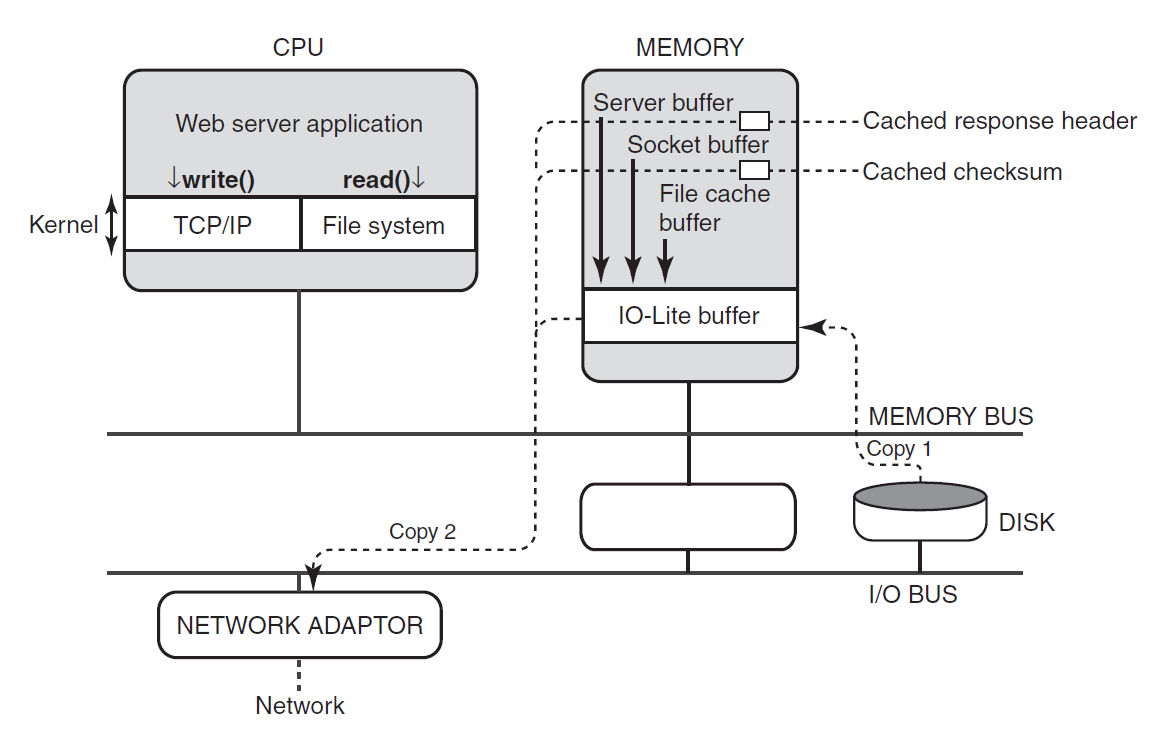
\includegraphics[width=\textwidth]{images/chap5/io_lite}

\textbf{Problems with file system integration:} 

\begin{itemize}
    \item Complex sharing patterns (application, network stack, file system all may point to buffer)
    \item Page can be VM Page and also File Page, hence complex replacement policy needed (standard page replacement and file cache replacement)
    \item Going over an OS (Unix) requires clean way of integration without major changes to the underlying OS
\end{itemize}

The graphic shows the base idea, I don't think we need to know more detail.

\subsection{Avoid file system copies via I/O splicing}

\textbf{IO-Splicing} is used to get rid of all copies we've seen before. Basically, the data goes directly from the file cache buffer to the network adaptor without any intermediary steps. Systems probide calls such as \texttt{sendfile()}, which does exactly that.


















\chapter{Control Overhead} \label{CHAP:CTLOVERHEAD}

[WIP]

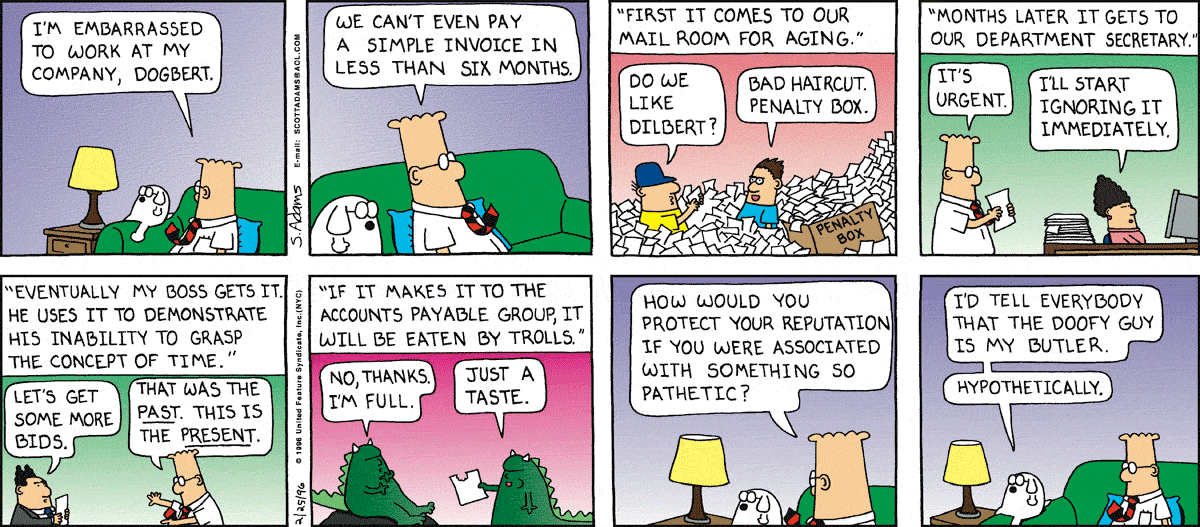
\includegraphics[width=\textwidth]{images/chap6/dilbert.png}

\section{What is Control Overhead?}

If a modern CPU processes a network message it goes through different layers of mediation.  The device, for example, an Ethernet adaptor, \textit{interrupts} the CPU, asking somewhat
stridently for attention. Control is passed to the kernel. The kernel batches interrupts wherever possible, does the network layer processing for the packet, and finally \textit{schedules} the application process (say, a Web server) to run. The web server creates new processes/threads, read/write files (\textit{system call}) and sends out the HTTP response by writing to the corresponding connection (another system call).

Thus an unoptimized implementation can incur considerable process-switching overhead
(hundreds of microseconds) if the application and networking code is poorly structured. Even
if process-structuring overhead is removed, system calls can cost tens of microseconds, and
interrupts can cost microseconds. To put these numbers in perspective, observe that on a 10-GB Ethernet link, a 40-byte packet can arrive at a PC every 3.2 µsec.





\section{Getting Rid of Control Overhead}

This section describes how to reduce control overhead costs, from the largest (context switches) to the smallest (interrupt overhead).

\subsection{Context switches}

In what follows, we will use a Web server as an example of a canonical server that may require the handling of a large number of connections. To do this efficient the server has to take every opportunity for concurrency

We now consider various ways to structure a server application and their effects on concurrency and scheduling overhead.

\subsubsection{Process per Client}

For every client the web server creates a new process. This results in the following advantages and disadvantages:

\begin{itemize}
\item[$\oplus$] OS scheduler juggles between clients
\item[$\circleddash$] process-context switching is expensive
\item[$\circleddash$] spawning a new process is also expensive
\item[$\circleddash$] matchmaking between new arriving clients and processes in pool
\end{itemize}


\subsubsection{Thread per Client}

Threads share the same virtual memory and generally trust each other, as is appropriate for all the threads processing different clients in a web server.

\begin{itemize}
\item[$\oplus$] common cache
\item[$\oplus$] smaller overhead than process per client
\item[$\circleddash$] still considerable overhead (e.g. save/restore stacks and registers)
\end{itemize}


\subsubsection{Event-Driven Scheduler}

If a general-purpose operating system facility is too expensive, the simplest strategy is to avoid
it completely. Thus while thread scheduling provides a facility for juggling between clients
without further programming, if it is too expensive, the application may benefit from doing
the juggling itself. Effectively, the application must implement its own internal scheduler that
juggles the state of each client.

\begin{center}
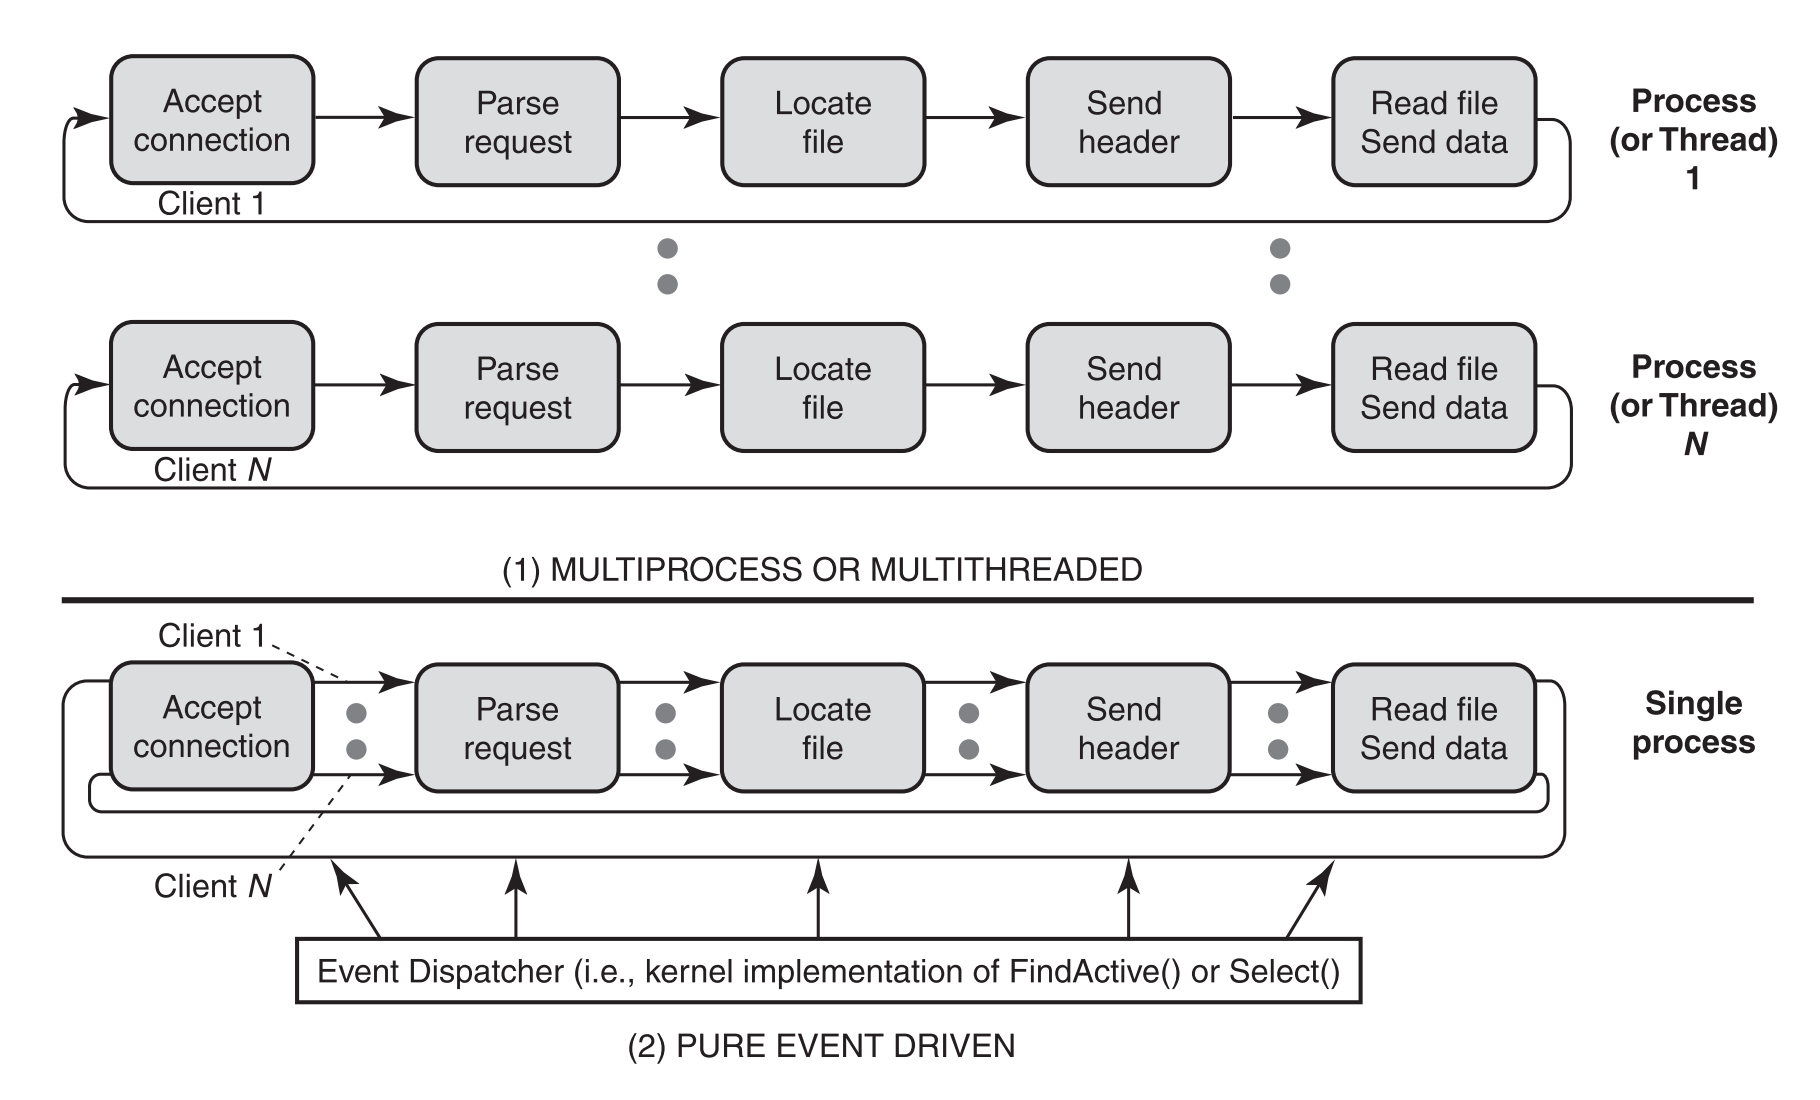
\includegraphics[width=.7\textwidth]{images/chap6/multiprocess-event.png}
\end{center}

The main idea is that the application stays in a loop invoking the FindActive()\footnote{This is a generic term. e.g. UNIX provides the select() system call.} call, which returns a list of all completed I/O descriptors. Assuming there is always some work to do on behalf of some client, the call will return with a list of I/O descriptors (e.g., file 1 data is now in memory, connection 5 has received data) with pending work. When the Web server processes these active descriptors, it loops back to making another FindActive() call.

\begin{itemize}
\item[$\oplus$] internal scheduling is more efficient
\item[$\circleddash$] requires non-blocking disk operations
\end{itemize}


\subsubsection{Event-Driven Server with Helper Processes}

The difficulty is that many operating systems, such as Solaris and UNIX, allow nonblocking read() and write() operations on network connections but may block when used on disk
files. Thus in such operating systems one must choose between the loss of concurrency incurred by blocking on disk I/O and going beyond the single-process model.

To avoid this problem, blocking operations are outsourced to helper processes.



\subsection{System calls}

When the application wants to receive data, it must specify buffers where the received
packet data should be written to. Today, in UNIX this is typically done using system calls,
where the application tells the kernel about data it wishes to send and buffers it wishes to receive to.

This appears to be required because there can be several applications sending and receiving
data from a common adaptor; since the adaptor is a shared resource, it seems unthinkable for an application to write directly to the device registers of a network adaptor without kernel mediation to check for malicious or erroneous use. Or is it?

Analogous to memory pages, our application can allocate adaptor pages and read/write descriptors directly to them without bothering the kernel. A descriptor is a small piece of information that describes the buffer in main memory where the data for the next packet should be written to. When a new packet arrives for the web application, the adaptor will demultiplex the packet on the basis of those descriptors.


\subsection{Interrupts}

There is no way to avoid interrupts completely. However, one can reduce interrupt overhead using the following tricks.

\begin{itemize}
\item \textbf{Interrupt only for significant events} e.g. only for the first packet received in a stream of packets.

\item \textbf{Polling} CPU keeps checking to see if packets have arrived.

\item \textbf{Application controlled} The sender is able to control when the receiver interrupts by passing a bit in the packet header.
\end{itemize}

\chapter{Timers} \label{CHAP:TIMERS}

\section{Motivation: Why Timers?}

Examples where timers are needed:
\begin{itemize}
\item repetitive tasks of
	\begin{itemize}
	\item the client: VoIP, multimedia player, ...
	\item the server: refresh of pages, speed for streaming, ...
	\end{itemize}
\item timeouts
\item scheduling
\item flow control
\item message acknowledgements
\item failure recovery
\end{itemize}
$\Rightarrow$ a large number of timers with fine granularity is needed

\section{Different timers}

Precondictions: 
\begin{itemize}
\item the maximum possible interval is known (given by the storage used for an interval, e.g. $32$ bit results in maximum interval $2^{32}$)
\item the intervals are represented by integers
\end{itemize}

Supported operations:
\begin{itemize}
\item startTimer(interval, id, expiryAction): inserts the timer
\item stopTimer(id): removes the timer
\item perTickBookkeeping(): checks for expired timers (and calls stopTimer(id))
\item expiryProcessing(): calls the expiryAction-method
\end{itemize}

\subsection{Timing Wheels}

General idea: hash the timers into buckets with their interval as key.

\subsubsection{Hashed Wheels}

Idea: the first $x$ bits are hashed into buckets, the remainder is inserted into a sorted linked list.\\

Costs refer to the worst-case running time for one method call, where $n$ is the overall number of timers and $n(t) \leq n$ denotes the number of expired timers at the moment $t$.\\
\begin{tabular}{p{0.2\linewidth}|p{0.6\linewidth}|p{0.2\linewidth}}
Method & Action & Costs \\
\hline \hline
startTimer & hash the timer into a bucket using $x$ higher order bits of its interval; insert the timer into a sorted linked list (ordered by expiration) & $O(n)$ since we have to traverse the whole list\\
perTickBookkeeping & calculate the bucket of the current time; expire all timers in the list until we reach the first timer, that expires later; we can stop since the list is sorted & $O(n(t))$ which is optimal \\
\end{tabular}\\
For stopTimer we store a pointer to the timer and use a doubly linked list, then we can remove it in $O(1)$.\\

Conclusion: 
\begin{itemize}
\item fast perTickBookkeeping
\item slow insertion, especially if many timers are in one bucket and thus the sorted linked list is large
\end{itemize}

\subsubsection{Hierarchical Wheels}

Idea: use different arrays at different precision levels and look at the timer in detail only if you need to do so because it expires soon.\\
(Note that we can calculate how many levels we need, because we know the maximum interval that is possible.)\\

Example:\\
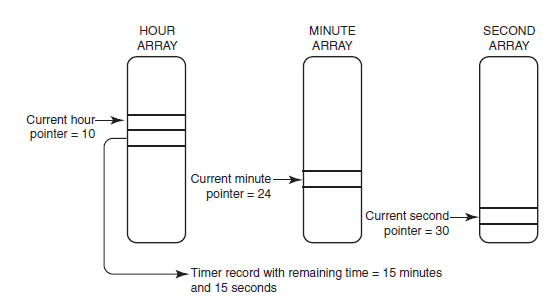
\includegraphics[width=0.5\linewidth]{images/chap7/hierarchicalTimingWheel.png}\\
To add a timer that expires in $5$ seconds, i.e. at $10:24:45$, we insert it directly into the Second Array.\\
To add a timer that expires in $3$ minutes, i.e. at $10:27:30$, we insert it into the Minute Array, since minutes is the highest level on which the value isn't equal to the current time.\\
When the current time points to $27$ all entries of this bucket are inserted into the Second Array.\\

\begin{tabular}{p{0.2\linewidth}|p{0.6\linewidth}|p{0.2\linewidth}}
Method & Action & Costs \\
\hline \hline
startTimer & hash the timer into the right bucket on the right level (highest level where current time and timer interval are not equal); insert it as first timer into the list of timers there & $O(1)$ which is optimal\\
perTickBookkeeping & expire and remove all timers in the current bucket at the lowest level; if the current time reached the end of an array, update levels from the next higher level (continue if necessary until highest level), i.e. take the current bucket and hash its timers to the lower level &  $O(n)$ since we have to traverse the lists of all levels in the worst-case and they may consist of all timers \\
\end{tabular}\\

Conclusion: 
\begin{itemize}
\item fast insertion
\item slower perTickBookkeeping, but only if the current time reaches the end of an array and every timer is touched maximal once for each level
\end{itemize}

Note: if precision of timers is allowed to decrease with higher levels, we don't have to update the timers into a different level.

\subsection{BSD implementation}

$200$ msec timers are used.\\

In the BSD implementation the method to stop the timer cannot take a pointer as argument.\\
Two possible solutions:
\begin{itemize}
\item define a new function which takes a pointer as argument
\item or use a hash table to search the callout for a given function
\end{itemize}

\subsection{Soft timers}

Problem: perTickBookkeeping can only be called as often as the timer ticks, thus we need fine granular timers. \\
Normal is around $1$ msec. If we want to achieve finer granularity, we could use a programmable harware interrupt chip (provided by most CPUs). But this causes a lot of overhead, ~$45$\%, because the CPU state (i.e. registers, TLB, ...) has to be stored on each interrupt.\\

Solution: Use other transition events, that include saving the CPU state anyway (e.g. system calls, exceptions, hardware interrupts), and add a timer interrupt there. \\
But we trade precision for speed, since usually such an event takes place every $10 \mu$sec, but it is not guaranteed.\\
In order to guarantee a worst-case of $1$ msec, we could add a hardware clock interrupt every $1$ msec.
\chapter{Exact-Match Lookups} \label{CHAP:EXMATCH}

What is an exaxt-match lookup?
\begin{itemize}
\item simplest form of database query
\item set of tubles: key K and state information
\item can use binary search and hash tables
\end{itemize}
\textbf{Ethernet under fire}
\\
\\
They are still interesting for this topic because different to the "usual" algorithmic setting, because they need to finish the search in time to receive a packet, they use memory references as a measure of speed and the potential use of hardware speedups. They are also important for bridging.\\
\\
Bridges were designed to "extend" a single Ethernet. They would work with the data link layer, which contains a 48-bit unique Ethernet destination address.\\
\\
The path to the final resolution:
\begin{itemize}
\item \textbf{Packet Repeater:} picks up entire packets, buffers them and sends them to the other Ethernet port. Distance span is increased to 3km but bandwidth doesn't change.
\item \textbf{Filtering Repeater:} Repeater has a table that maps station addresses to Ethernets. Only packets which need repeating are repeated. If a fraction p of the traffic has a destination on the same Ethernet, the bandwidth (1+p) and distance increases. Only problem is building the table.
\item \textbf{Filtering Repeater with Learning:} The bridge also looks on the source address and starts building it's mapping table.
\end{itemize}
\textbf{Wire Speed Forwarding}
\\
Problem with the last idea is, that if the bridge takes more time to analyze a packet (check the mapping table), than to receive a packet, some packets may be discarded since the buffer is full. Thus an implementation with wire speed forwarding was proposed.\\
\\
The bridge only had 51.2 $\mu $sec to forward a packet. This means both lookups (destination for forwarding and source for learning) had to be done within 25.6 $\mu $sec. The first design consisted f a processor, two Ethernet chips, a lookup chip and a four-ported memory, which could be read and written by the processor, the Ethernet chips and the lookup engine.\\
\\
The design worked with:
\begin{itemize}
\item \textbf{Architectural Design}: Memory was cheap DRAM with a cycle time of 100 nsec. It was designed to maximize parallelism and minimize interference so the processor can still work, while the lookup engine worked.
\item \textbf{Data Copying}: The Ethernet chips used DMA to place packets in the memory without processor control. Later only a pointer needed to be flipped to change a packet from receive to transmit queue.
\item \textbf{Control Overhead}: To minimize overhead the processor used polling, staying in a loop after a packet interrupt. Whe  the receive queues are empty the processor does other chores.
\item \textbf{Lookups}: Used binary search but software lookup exceeded 25.6 $\mu $sec. Added hardware with combinatorial logic made it possible to use a mapping table of 8000 entries within a lookup time of 1.3 $\mu $sec.
\end{itemize}
\textbf{Scaling Lookups to Higher Speeds}\\
\\
The popularity of bridges led to an increase of the lookup table from 8K entries to 64K entries. This means binary search would need 16 memory access which would take 3.2 $\mu $sec with DRAM. for 40 byte packets this would be too slow.\\
\\
One alternative would be to use SRAM, which is 5-10 times faster than DRAM. But this was expensive and would not work for the next speed increment.\\
\\
So \textit{Scaling via Hashing} was the solution. The idea of the Gigaswitch was used to design a FDDI-to-Gigaswitch network controller. It used perfect hashing. With a parameterized hash function it was possible to have only four memory access in the worst case within the 64K lookup table.\\
\\
An alternative approach was \textit{Hardware Parallelism}. It pipelines the binary search to increase the lookup throughput. 
\chapter{Prefix-Match Lookups} \label{CHAP:PREFMATCH}

For Prefix-Match Lookups bits are used. The 116-bit IP prefix 132.239 would be 1000010011101111* for example. Another denotation would be 123.239.0.0/16 which shows only the first 16 bits are relevant. The third notation uses a mask. 132.239.0.0 with a mask of 255.255.0.0 shows again that only the first 16 bits matter since 255.255.0.0 only has 1's in the first 16 bits.

\textbf{Why Variable-Length Prefixes}

In general: They make more use of the address space.\\
\\
In specific: The internet began with a hierarchy in which 32-bit addresses were divided into a network address and a host number. This lead to a classification (Class A: 8 bits, Class B: 16 bits, Class C: 24 bits) of the address space. In today's world small companies may be only given a small part of a Class C address, maybe a /30, which lead to schemes like network address translation (NAT)

\textbf{Lookup Model}

Observations:
\begin{itemize}
\item \textbf{1}: Caching solutions won't work because of the large number of flows.
\item \textbf{2}: Lookup needs to be done at wire speed, since many packets are minimum-sized.
\item \textbf{3}: Measure of speed is worst case of memory accesses.
\item \textbf{4}: Naive schemes will require 24 memory accesses in worst case since prefix lengths wary from 8 to 32.
\item \textbf{5}: Future backbone routers will have prefix databases of 500,000 to 1 million prefixes.
\item \textbf{6}: Unstable routing-protocol implementations may lead to updates of the lookup table in the order of miliseconds. This is several orders of magnitude below lookup requirements, allowing a more complex updating in order to speed up lookup.
\item \textbf{7}: Another metric is memory usage (DRAM vs SRAM)
\item \textbf{8}: At the time of writing 32-bit IP addresses were the most interesting
\end{itemize}

\textbf{Finessing Lookups}

\textbf{Threaded Indices and Tag Switching}

With this method every packet gets information of the next routing table in it's header. This means lookup take only one memory access, No Prefix-matching is necessary since the position of the entry for the next hop is already known through the information in the header.

This means the routers need to precompute the routing tables every time the topology changes and send their distance and index for every of their neighbours to all of their neighbours.

\textbf{Flow Switching}

Flow Switching also works with passing an index to the next hop, but different to Tag Switching it is computed on demand. The "second" router decides to switch packets if it notices a lot of traffic. It sends an idle virtual circuit identifier to the "first" router and maps this identifier to the outgoing port. Now every packet which comes from the "first" router and is labelled with this identifier will be send to the right port without the need of a lookup.
\chapter{Additional Stuff} \label{CHAP:ADD}

\textbf{Memory and Hardware:}

\textbf{SRAM:} Static RAM using flip-flops for feedback loops. Access in 0.5 to 1 nsec.

\textbf{DRAM:} Dynamic RAM, cheaper stores in flip-flop with output capacitance, possibly leaking. Refresh necessary, hence slower.

\textbf{Memory Subsystem Design techniques:}
\begin{itemize}
    \item Memory Interleaving and piepelining
    \item Wide word parallelism
    \item Combination of DRAM and SRAM
\end{itemize}

\textbf{Hardware:} Chip Complexity Scaling (Double components every 2 years), Chip Speeds, Chip I/O (slow increase in pins on chip), Serial I/O (Chip to Chip), Memory Scaling (Access times), Power and Packaging..

\textbf{Network Device Architectures:}

\textbf{Endnodes:} Workstations and so on, Needs external DRAM, speeding up CPU using caches (L1 SRAM, L2 SRAM, uses simple hashes), I/O is memory mapped (NA and Disk look like memory), \textbf{DMA}. Adapters on I/O bus (backwards compatible, i.e., PCI).

\textbf{Routers:} Set of input/output links, needs switching and lookup (consults \textbf{FIB} with LPM), after lookup -> internal switching (I-link to O-link).. and also needs queuing (FIFO if link is congested), Header Validation and Checksums (TTL, IP Checksum, MAC CRC), Protocol processing (SNMP for statistics, ARP synchrionization and more).

\textbf{Virtual Memory:} "Infinite Memory", Mapping of Logical addresses to physical space (can use disk space as memory).

\textbf{Networking:}

\textbf{Protocols:} Ethernet Link layer protocol (MTU ~1500bytes) , uses MAC addresses, Header 14+4 bytes:

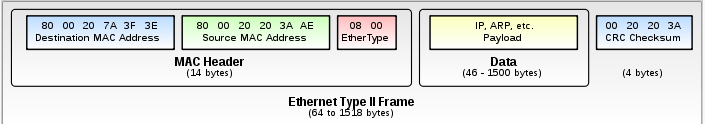
\includegraphics[width=.8\textwidth]{images/chap10/ethernet_header}

\textbf{CRC:} Cyclic redundancy check, basically a hash, can be computed by hardware. Uses polynomial with n-bit order to encode coefficients.

\textbf{IP}: Internet Protocol, used for routing, needs checksum (16 bit, uses TTL, changes every HOP, all 16-bit words in header added up based on ones-complement), Hedaer 20 Bytes + Options:

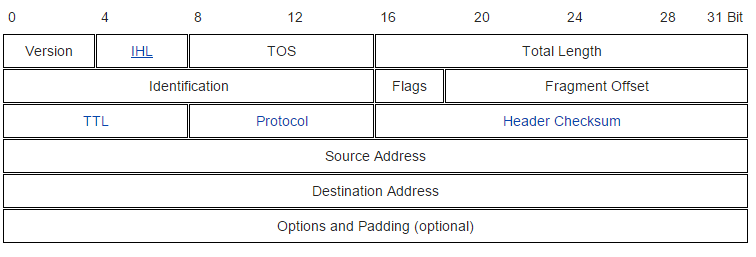
\includegraphics[width=.7\textwidth]{images/chap10/ip_header}

\textbf{TCP:} Transmission Control, Connection-oriented, uses SYN/ACK for state, Checksum (16bit, Uses IP-pseudoheader: SRC/DEST Address, Null-Byte, Val 6 for TCP, TCP Length, pseudoheader not sent), Use slow-start (increase congestion windows with every ACK received, exponential, until slow-start threshold reached or if timeout half threshold and set congestion window to 1), Header 20 - 24 Byte:  

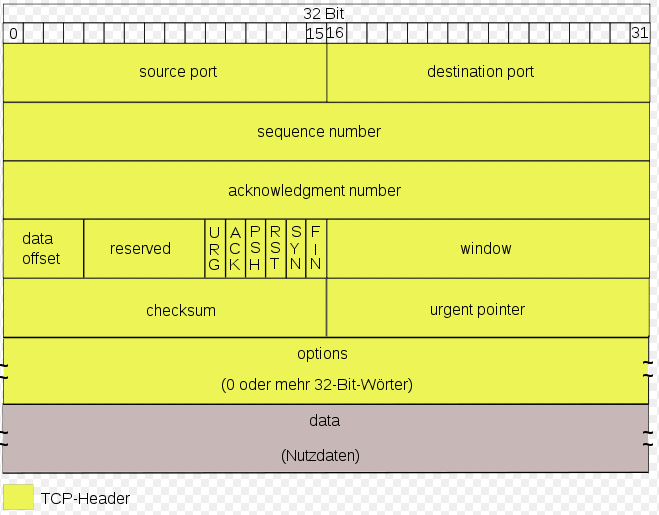
\includegraphics[width=.7\textwidth]{images/chap10/tcp_header}

Minimum Size internet packet: 14+4 + 20 + 20 + 24 = ~60 bytes!


\end{document}